\begin{appendices}
\chapter{Appendix: Chapter 2}
\section{Example of a non-basis independent ``trace''}\label{app:bad-sum-is-bad}
Consider an infinite dimensional Hilbert space spanned by basis vectors $\left\{\ket{e_k}\middle|k\in\N\right\}$. Let $Z$ be the operator acting as
\begin{align}
  Z\ket{e_{2n}} &= \ket{e_{2n}}\\
  Z\ket{e_{2n+1}} &= -\ket{e_{2n+1}},
\end{align}
effectively the direct sum of Pauli-z operators acting in two dimensional subspaces. For $k\in\N$ define the operators $U_{k\theta}$ acting as rotations around the $y$ axis in the $k^\text{th}$ two dimensional subspace, and the identity outside
\begin{align}
  U_{k\theta} \ket{e_{2k}} &= \cos(\theta) \ket{e_{2k}} + \sin(\theta)\ket{e_{2k+1}}\\
  U_{k\theta} \ket{e_{2k+1}} &= -\sin(\theta) \ket{e_{2k}} + \cos(\theta)\ket{e_{2k+1}}\\
  U_{k\theta} \ket{e_k} &= \ket{e_j},                            
\end{align}
where $j\neq 2k, 2k+1$, then 
\begin{align}
  \braket{U_{k\theta}e_{2k}}{ZU_{k,\theta}e_{2k}} &= \cos^2(\theta) - \sin^2(\theta)\\
  \braket{U_{k\theta}e_{2k+1}}{ZU_{k,\theta}e_{2k+1}} &= -\cos^2(\theta) + \sin^2(\theta).
\end{align}
We choose $\theta_k$ such that 
\begin{align}
  \braket{U_{k\theta_k}e_{2k}}{ZU_{k,\theta_k}e_{2k}} = \frac{1}{k+1} = -\braket{U_{k\theta_k}e_{2k+1}}{ZU_{k,\theta_k}e_{2k+1}}.
\end{align}
If the basis $\left\{\ket{\phi_k}\middle|k\in\N\right\}$ is chosen such that 
\begin{align}
  \ket{\phi_{2k}} &= U_{k,\theta_k}e_{2k}\\
  \ket{\phi_{2k+1}} &= U_{k,\theta_k}e_{2k+1},
\end{align}
then we can rewrite the terms of the series
\begin{align}
  \sum_{k\geq 0} \braket{\phi_k}{Z\phi_k} = \sum_{k>0}\frac{(-1)^{k-1}}{\lfloor k/2\rfloor},
\end{align}
where $\lfloor x\rfloor$ denotes the \emph{floor} of $x$, the largest natural below $x$. It is now easy to see the series converges to zero, but does not converge absolutely. By the Riemann series theorem \cite{Sierpinski1910} this series may be rearranged (by relabelling basis elements) to give any real number as the sum.

\chapter{Appendix: Chapter 3}

\section{Uncertainty region for Gell-Mann observables}
\label{app:gellmann-ur}
Given
\begin{align}
  \opa = \begin{pmatrix}
    1 & 0 & 0\\
    0 & -1 & 0\\
    0 & 0 & 0\\
  \end{pmatrix} \quad
  \opb = \begin{pmatrix}
    0 & 0 & 1\\
    0 & 0 & 0\\
    1 & 0 & 0\\
  \end{pmatrix} \quad
  \rho =\begin{pmatrix}
    \rho_{11} & 0 & \rho_{13}\\
    0 & 1-\rho_{11} - \rho_{33} & 0\\
    \rho_{13}^* & 0 & \rho_{33}
  \end{pmatrix},
\end{align}
we can solve
\begin{align}
  x &= \varr{\opa}\\
    &= 1 - \rho_{33} - \left(2\rho_{11} + \rho_{33} - 1\right)^2,
\end{align}
giving
\begin{align}
  \rho_{33}^\pm = \frac{1}{2}\left(1-4\rho_{11} \pm\sqrt{1+8\rho_{11}-4x}\right).
\end{align}
The positivity of $\rho$ constrains the choice of $\rho_{11}$ values in each case. If
\begin{align}
  \rho^\pm = \begin{pmatrix}
    \rho_{11} & 0 & \rho_{13}\\
    0 & 1-\rho_{11} - \rho_{33}^\pm & 0\\
    \rho_{13}^* & 0 & \rho_{33}^\pm
  \end{pmatrix}
\end{align}
and $0\leq\rho_{13}\leq\sqrt{\rho_{11}\rho_{33}}$ then
\begin{align}
  \label{eqn:rho-plus-constraints}
  \rho^+ \geq 0 &\iff \begin{cases}\left[ 0\leq \rho_{11}\leq\frac{1}{2}(1-\sqrt{1-4x})\right] \text{ or } \left[\frac{1}{2}(1+\sqrt{1-4x})\leq\rho_{11}\leq\frac{1}{2}(1+\sqrt{1-x})\right],  &0\leq x\leq\frac{1}{4}\\
    \frac{1}{8}\left(4x-1\right)\leq \rho_{11}\leq \frac{1}{2}\left(1+\sqrt{1-x}\right), & \frac{1}{4}\leq x\leq \frac{3}{4}\\
    \frac{1}{2}\left(1-\sqrt{1-x}\right)\leq \rho_{11} \leq\frac{1}{2}(1+\sqrt{1-x}, & \frac{3}{4}\leq x\leq 1
  \end{cases}\\ 
  \rho^- \geq 0 &\iff \begin{cases}0\leq\rho_{11}\leq\frac{1}{2}(1-\sqrt{1-x}), &0\leq x\leq\frac{1}{4}\\
    \frac{1}{8}\left(4x-1\right)\leq\rho_{11}\leq\frac{1}{2}(1-\sqrt{1-x}), & \frac{1}{4}\leq x\leq \frac{3}{4}\\
    \text{no valid solution}, & \frac{3}{4}\leq x\leq 1.
  \end{cases}\label{eqn:rho-minus-constraints}
\end{align} %$
The constraints on $\rho_{13}$ imply that $0\leq\left(\Re{\rho_{13}}\right)^2\leq\rho_{11}\rho_{33}^\pm$. Obviously $\var[\rho^\pm]{\opb}$ will be minimised by a $\rho^\pm$ with $\left(\Re{\rho_{13}}\right)^2 = \rho_{11}\rho_{33}^\pm$ and maximised when $\left(\Re{\rho_{13}}\right)^2 = 0$.
\begin{align}
  \var[\rho^\pm]{\opb} = \rho_{11} +\rho_{33}^\pm - 4\lambda\rho_{11}\rho_{33}^\pm.
\end{align}
For a fixed $x$ the local minima and maxima will either be where the inequalities above are saturated or where the derivative of $\var[\rho^\pm]{\opa}$ with respect to $\rho_{11}$ (considering $\rho_{33}^\pm$ as a function of $\rho_{11}$) is zero. 

\subsection{Exploring minima}
Here we consider the case $\left(\Re{\rho_{13}}\right)^2 = \rho_{11}\rho_{33}^\pm$. In this case
\begin{align}
  \var[\rho^\pm]{\opb} &= \rho_{11} + \rho_{33}^\pm -4\rho_{11}\rho_{33}^{\pm}\\
                       &= \frac{1}{2}\left(1 -6\rho_{11} + 16\rho_{11}^2 \pm (1-4\rho_{11})\sqrt{1+8\rho_{11}-4x}\right)\\
  \diff{\left(\var[\rho^\pm]{\opb}\right)}{\rho_{11}} &= -3 + 16\rho_{11} \mp 2\sqrt{1+8\rho_{11}-4x}\pm \frac{2-8\rho_{11}}{\sqrt{1+8\rho_{11} -4x}}\\
  \diff{\left(\var[\rho^\pm]{\opb}\right)}{\rho_{11}} &= 0 \iff (3 - 16\rho_{11})\sqrt{1+8\rho_{11} -4x} =\pm \left(8x-24\rho_{11}\right).
                                                        \label{eqn:deriv-y-rhomin-is-zero}
\end{align}
The solutions to this equation obey a cubic equation
\begin{align}
  (3 - 16\rho_{11})^2(1+8\rho_{11} -4x) &=\left(8x-24\rho_{11}\right)^2\\
  0&= (32 \rho_{11}-16 x+3) (8 \rho_{11} (8 \rho_{11}-5)+4 x+3),
\end{align}
with solutions
\begin{align}
  \rho_{11}^\pm &= \frac{1}{16} \left(5\pm\sqrt{13-16 x}\right)\\
  \rho_{11}^0 &= \frac{1}{32} \left(16 x-3 \right).
\end{align}
Substituting these back into \eqref{eqn:deriv-y-rhomin-is-zero} we see that $\rho_{11}^0$ and $\rho_{11}^+$ are solutions wherever they give valid quantum states, but $\rho_{11}^-$ is only a solution if $x=\frac{9}{16}$ or $\frac{3}{4}\leq x$. Comparing the solutions with the restrictions \eqref{eqn:rho-plus-constraints} we get the following solutions for $\rho^+$, and no solutions for $\rho^-$
\begin{subequations}
\label{eqn:rho-plus-zero-deriv-solns}
\begin{align}
  \rho_{11} = \frac{1}{32} \left(16 x-3 \right) &\text{ on } x\in\left[\frac{3}{16}, \frac{15}{16}\right]\\
  \rho_{11} = \frac{1}{16} \left(5+\sqrt{13 - 16x} \right) &\text{ on } x\in\left[\frac{9}{100},\frac{13}{16}\right]\\
  \rho_{11} = \frac{1}{16} \left(5-\sqrt{13 - 16x} \right) &\text{ on } x\in \left\{\frac{9}{16}\right\}\cup\left[\frac{3}{4},\frac{13}{16}\right],
\end{align}
\end{subequations}
note that the apparently exceptional point $x = \frac{9}{16}$, $\rho_{11} = \frac{3}{16}$ lies on the line $\rho_{11} = \frac{1}{32} \left(16 x-3 \right)$. To these we add the boundary values
\begin{subequations}
\label{eqn:rho11-con}
\begin{align}
  \label{eqn:rho-plus-con-1}\rho_{11} = 0 &\text{ with } \rho_{33}^+ \text{ and } x\in\left[0,\frac{1}{4}\right]\\
  \label{eqn:rho-plus-con-2}\rho_{11} = \frac{1}{2}\left(1-\sqrt{1-4x}\right) &\text{ with } \rho_{33}^+ \text{ and } x\in\left[0,\frac{1}{4}\right]\\
  \label{eqn:rho-plus-con-3}\rho_{11} = \frac{1}{2}\left(1+\sqrt{1-4x}\right) &\text{ with } \rho_{33}^+ \text{ and } x\in\left[0,\frac{1}{4}\right]\\
  \label{eqn:rho-plus-con-4}\rho_{11} = \frac{1}{2}\left(1+\sqrt{1-x}\right) &\text{ with } \rho_{33}^+ \text{ and } x\in\left[0,1\right]\\
  \label{eqn:rho-plus-con-5}\rho_{11} = \frac{1}{8}\left(4x-1\right) &\text{ with } \rho_{33}^+ \text{ and } x\in\left[\frac{1}{4},\frac{3}{4}\right]\\  
  \label{eqn:rho-plus-con-6}\rho_{11} = \frac{1}{2}\left(1-\sqrt{1-x}\right) &\text{ with } \rho_{33}^+ \text{ and } x\in\left[\frac{3}{4},1\right]\\
  \label{eqn:rho-minus-con-1}\rho_{11} = 0  &\text{ with } \rho_{33}^- \text{ and } x\in\left[0,\frac{1}{4}\right]\\
  \label{eqn:rho-minus-con-2}\rho_{11} = \frac{1}{8}(4x-1)  &\text{ with } \rho_{33}^- \text{ and } x\in\left[\frac{1}{4},\frac{3}{4}\right]\\
  \label{eqn:rho-minus-con-3}\rho_{11}= \frac{1}{2}(1-\sqrt{1-x}) &\text{ with } \rho_{33}^- \text{ and } x\in\left[0,\frac{3}{4}\right]\
\end{align}
\end{subequations}
the (locally) extremising values of $\rho_{11}$ are summarised in Figure \ref{fig:rho-plus-vals}. The values of $\var[\rho_{11}^+]{\opb}$ given these choices of $\rho_{11}$, and $\left(\Re{\rho_{13}}\right)^2 = \rho_{11}\rho_{33}^\pm$ are plotted in Figure \ref{fig:rho-minus-vals}.
\begin{figure}[ht]\centering
  \begin{subfigure}[t]{0.4\textwidth}
    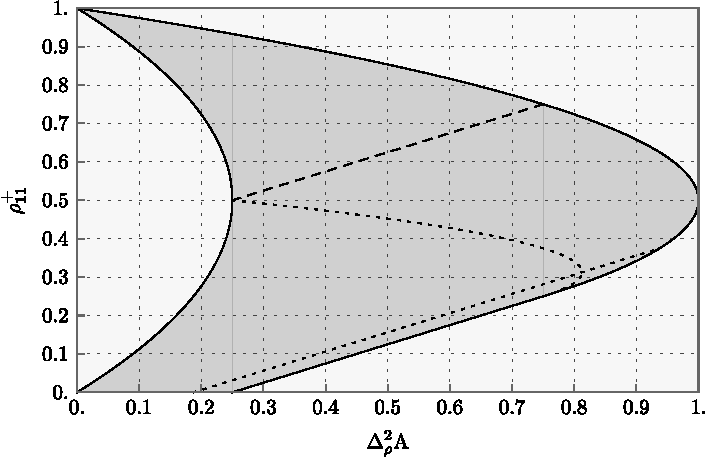
\includegraphics[height=0.65\linewidth]{figs/qutrit-rhoplus-r11vals}
    \caption[Range of $\rho_{11}$ given $\rho_{33} = \rho_{33}^+$]{Range of $\rho_{11}$ given $\rho_{33} = \rho_{33}^+$. The dotted lines are the where $\Re{\rho_{13}}$ is maximal and the derivative of $\var[\rho^+]{\opb}$ with respect to $\rho_{11}$ is zero \eqref{eqn:rho-plus-zero-deriv-solns}, the dashed line is the where $\Re{\rho_{13}} = 0$ and the derivative of $\var[\rho^+]{\opb}$ with respect to $\rho_{11}$ is zero \eqref{eqn:rho-plus-max-zero-deriv-solns}.}\label{fig:rho-plus-vals}
  \end{subfigure}\quad
  \begin{subfigure}[t]{0.4\textwidth}
    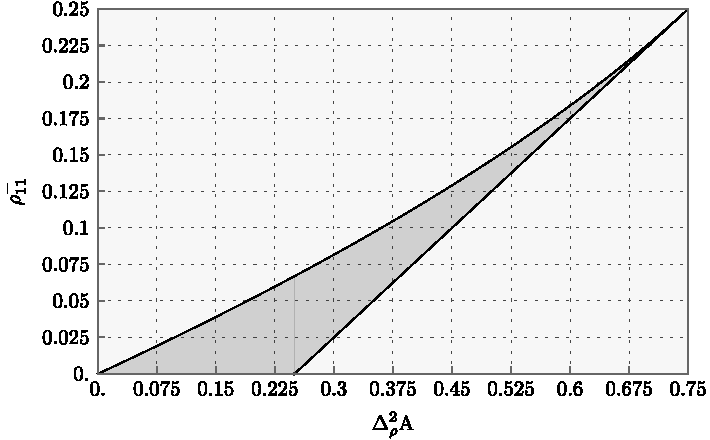
\includegraphics[height=0.65\linewidth]{figs/qutrit-rhominus-r11vals}
    \caption[Range of $\rho_{11}$ given $\rho_{33} = \rho_{33}^-$]{Range of $\rho_{11}$ given $\rho_{33} = \rho_{33}^-$. There are no local extrema other than the boundary curves.}\label{fig:rho-minus-vals}
  \end{subfigure}
  \caption[Allowed values of $\rho_{11}$ in the minimizing states for the Gell-Mann pair]{The filled region indicates the allowed values of $\rho_{11}$ as a function of $\var[\rho^+]{\opa}$ in each case. The solid lines are the boundary curves, given in  {\eqref{eqn:rho11-con}}.}
\end{figure}

\subsection{Exploring maxima}
Here we consider the case $\left(\Re{\rho_{13}}\right)^2 = 0$. In this case
\begin{align}
  \var[\rho^\pm]{\opb} &= \rho_{11} + \rho_{33}^\pm\\
                       &= \frac{1}{2} \left(1-2 \rho_{11}\pm\sqrt{8 \rho_{11}-4 x+1}\right)\\
  \diff{\left(\var[\rho^\pm]{\opb}\right)}{\rho_{11}} &= -1 \pm \frac{2}{\sqrt{8\rho_{11} -4x+1}}\\
  \diff{\left(\var[\rho^\pm]{\opb}\right)}{\rho_{11}} &= 0 \iff \sqrt{8\rho_{11} -4x+1} = \pm 2.
                                                        \label{eqn:deriv-y-rhomax-is-zero}
\end{align}
There are no solutions for $\rho_{33}^-$, but $\rho_{33}^+$ has the solution
\begin{align}
  \label{eqn:rho-plus-max-zero-deriv-solns}
  \rho_{11} = \frac{1}{8}\left(3+4x\right),
\end{align}
which is always a valid solution for $\rho^+$ and never valid for $\rho^-$. To this we add the boundary values which are the same as those with $\left(\Re{\rho_{13}}\right)^2 = \rho_{11}\rho_{33}$, given in \eqref{eqn:rho11-con}.

\subsection{The bounding curves}
Comparing the local extrema we can now describe the full uncertainty region shown in figure \ref{fig:qutrit-uncertainty-region}
\begin{alignat}{2}
  & \var{\opb} = 1, \quad && \var{\opa}\in\left[0,\frac{1}{4}\right]\\
  & \var{\opb} = \frac{1}{8} \left(9-4\,\var{\opa}\right), \quad && \var{\opa}\in\left[\frac{1}{4},\frac{3}{4}\right]\\
  & \var{\opb} = \frac{1}{2} \left(1+\sqrt{1-\var{\opa}}\right), \quad && \var{\opa}\in\left[\frac{3}{4}, 1\right]\\
  & \var{\opb} = \frac{1}{2} \left(1-\sqrt{1-\var{\opa}}\right), \quad && \var{\opa}\in\left[\frac{15}{16}, 1\right]\\ 
  & \var{\opb} =  2 \left(\var{\opa}\right)^2-\frac{11}{4}\,\var{\opa}+\frac{153}{128} \quad && \var{\opa}\in\left[\frac{13}{16},\frac{15}{16}\right]\\
  & \var{\opb} = \frac{1}{8} \left(4\,\var{\opa}-1\right), \quad && \var{\opa}\in\left[\frac{1}{4}, \frac{13}{16}\right]\\
  & \var{\opb} = 1-\var{\opa}, \quad && \var{\opa}\in\left[\frac{15}{64},\frac{1}{4}\right]\\
  & \var{\opb} = \frac{1}{2}\left(1-\sqrt{1-\var{\opa}}\right) \quad && \var{\opa}\in\left[0,\frac{15}{64}\right]\\
  & \var{\opb} = \frac{1}{2} \left(1-\sqrt{1-4\,\var{\opa}}\right)\quad  && \var{\opa}\in\left[0,\frac{3}{16}\right]\\  
  & \var{\opb} = 1-4\,\var{\opa}, \quad && \var{\opa}\in\left[0,\frac{3}{16}\right].
  \label{eqn:gellmann-bounding-curves}
\end{alignat}


\end{appendices}